Further improvements that could be made to our model and where this research could be taken.

\begin{figure}[H]
\centering
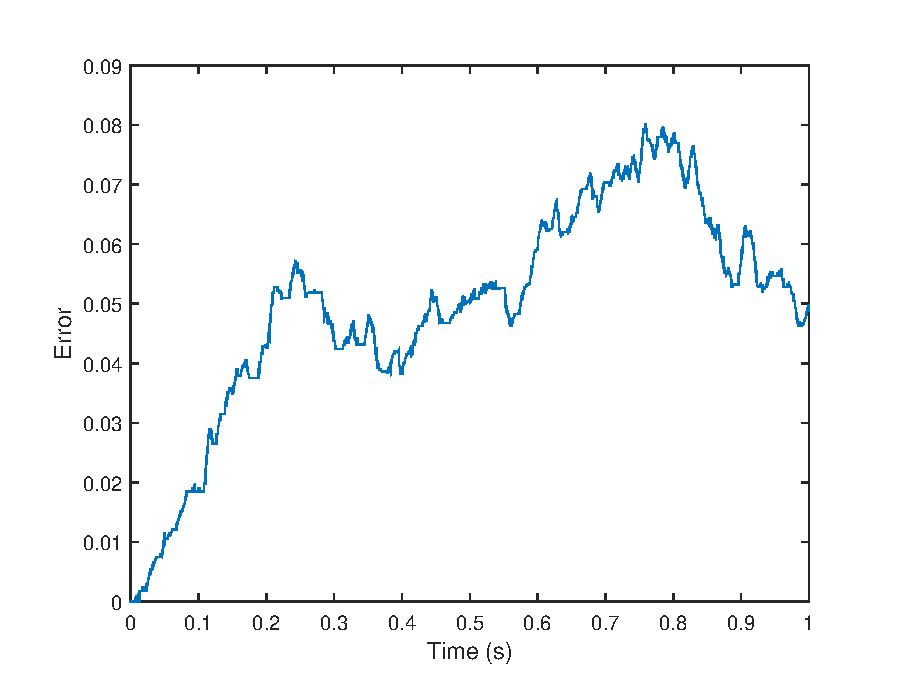
\includegraphics[width = \textwidth]{ErrorOverTime_6000Hz_perm_fixed.eps}
\label{EoT: fixed}
\caption{Here is a plot of error over time which was computed using the corrected algorithm presented in the methods section.}
\end{figure}